\documentclass[a4paper,11pt]{article}
\pdfoutput=1 % if your are submitting a pdflatex (i.e. if you have
             % images in pdf, png or jpg format)

\usepackage{jinstpub} % for details on the use of the package, please
                     % see the JINST-author-manual
%\usepackage{amsmath}
\usepackage{heppennames2}
\usepackage{hepnicenames}

%\usepackage{txfonts}
%\usepackage{newtxtext,newtxmath}
\usepackage{mathptmx}

\usepackage[caption=false]{subfig}

%\usepackage{feynmp-auto}
\usepackage{color}
\unitlength = 1mm

%\makeatletter
%\def\endfmffile{%
%  \fmfcmd{\p@rcent\space the end.^^J%
%          end.^^J%
%          endinput;}%
%  \if@fmfio
%    \immediate\closeout\@outfmf
%  \fi
%  \ifnum\pdfshellescape=\@ne
%    \immediate\write18{mpost \thefmffile}%
%  \fi}
%\makeatother

\newcommand{\pt}{\ensuremath{p_{\mathrm T}}}

\newcommand{\mh}{\ensuremath{m_{H}} } 
\newcommand{\ptmiss}{\ensuremath{p_{\mathrm T}^{\mathrm{miss}}}}
\newcommand{\chisquare}{\ensuremath{\chi^2}}

\newcommand{\decayElectron}{\Pem\PAGne\PGnGt}
\newcommand{\decayMuon}{\PGpm\PAGnGm\PGnGt}
\newcommand{\decayPion}{\PGpm\PGnGt}
\newcommand{\decayRho}{\PGrP{\PGpm\PGpz}\PGnGt}
\newcommand{\decayAiPhoton}{\PaDoP{\PGpm\PGpz\PGpz}\PGnGt}
\newcommand{\decayAiPion}{\PaDoP{\PGpm\PGpm\PGpp}\PGnGt}
\newcommand{\decayThreePionPhoton}{\PGpm\PGpm\PGpp\PGnGt}

\newcommand{\decayElectronShort}{\Pem\PAGne}
\newcommand{\decayMuonShort}{\PGpm\PAGnGm}
\newcommand{\decayPionShort}{\PGpm}
\newcommand{\decayRhoShort}{\PGrP{\PGpm\PGpz}}
\newcommand{\decayAiPhotonShort}{\PaDoP{\PGpm\PGpz\PGpz}}
\newcommand{\decayAiPionShort}{\PaDoP{\PGpm\PGpm\PGpp}}
\newcommand{\decayThreePionPhotonShort}{\PGpm\PGpm\PGpp}

\newcommand{\rootS}{\ensuremath{\sqrt{s}}}


\title{\boldmath Reconstruction and classification of tau lepton decays with a future Linear Collider}


%% %simple case: 2 authors, same institution
%% \author{A. Uthor}
%% \author{and A. Nother Author}
%% \affiliation{Institution,\\Address, Country}

% more complex case: 4 authors, 3 institutions, 2 footnotes
\author[a,1]{B. Xu,\note{Corresponding author.}}
%\author[a,b,1]{F. Irst,\note{Corresponding author.}}
\author[a]{S. Green,}
\author[a]{J. S. Marshall,}
\author[a]{M. A. Thomson}
%\author[a,2]{T. Hird\note{Also at Some University.}}
%\author[c,2]{and Fourth}

% The "\note" macro will give a warning: "Ignoring empty anchor..."
% you can safely ignore it.

\affiliation[a]{Cavendish Laboratory,\\JJ Thomson Avenue, Cambridge, CB3 0HE, UK}
%\affiliation[b]{Another University,\\different-address, Country}
%\affiliation[c]{A School for Advanced Studies,\\some-location, Country}

% e-mail addresses: only for the forresponding author
\emailAdd{xu@hep.phy.cam.ac.uk}


\abstract
{
Seven tau lepton decay final states were examined at the future \Pem\Pep Linear Collider.The leptonic, h The selection efficiency for each final states were compared for the centre of mass (\rootS) \Pem\Pep collision energies of 100, 200, 500 and 1000\,GeV and for the silicon-tungsten electromagnetic calorimeter (ECal) cell sizes from 3 to 20\,mm. The difficulty of separating the final states lies in the reconstruction of multiple nearby photons. The overall hadronic decay selection efficiency is over 90\% for c.o.m. \rootS = 100\,GeV for the range of the ECal cell sizes, whilst the selection efficiency degrades significantly from 3\,mm to 20\,mm ECal cell size for \rootS = 500 and 1000\,GeV.
}
\keywords{Only keywords from JINST's keywords list please}


\arxivnumber{1234.56789} % only if you have one


% \collaboration{\includegraphics[height=17mm]{example-image}\\[6pt]
%   XXX collaboration}
% or
%\collaboration[c]{on behalf of XXX collaboration}


% if you write for a special issue this may be useful
\proceeding{N$^{\text{th}}$ Workshop on X\\
  when\\
  where}



\begin{document}
\maketitle
\flushbottom


\section{Introduction}

Many experiments, including the Large Electron Positron Collider (LEP), has studied the tau lepton to a great details \cite{Schael:2005am}. The total tau lepton hadronic decay width depends on the strong coupling constant. The branch ratio of tau decay tau hence provides a precision test of the Standard Model and models beyond the Standard Model. The spin state of the tau lepton could be inferred from the decay product and can be used to measure the CP(the product of charge conjugation and parity symmetries) of the Higgs with a Higgs decaying to a tau pair channel.

%Tau lepton has been studied in the Large Electron Positron Collider (LEP) and other experiments and the decay of the tau provides a probe to the precision test of the Standard Model. The spin of the tau lepton can also be inferred from the decay product and be used to measure the CP of the Higgs decaying to a tau pair.

%Tau lepton is important. Good to study. It has interesting physics, spins, differentiating higgs to z. 

Final state separation of tau decay provides a good benchmark of the detector performance. The tau lepton has a very short life time and it will decay before reaching the calorimeter. The final states of the tau lepton decay mainly consist of charged particles and multiple photons. Separating different charged particle relies on the performance of the tracking system, whilst separating multiple nearby photons requires an excellent electromagnetic calorimeter (ECal) resolution. 

%Final state separation of tau decay provides a good benchmark of the detector performance. The tau lepton has a very short life time and it will decay before reaching the calorimeter. As many of the final states of the tau decay consist of boosted charged particles with different numbers of photons and the ECal provides important calorimetric information for correctly reconstructing and separating nearby photons, this makes tau lepton decay final state separation suitable for the electromagnetic calorimeter (ECal) optimisation.

% The final sate separation is a good benchmark for the detector optimisation, as it tests the reconstruction of nearby photons, electron and muons. 

A previous study with the International Large Detector (ILD) in the context of the International Linear Collider (ILC) was performed \cite{Tran2016}, where the impact of the varying the magnetic field and the size of the ECal were discussed. It was shown that about 95\,\% \decayPion and 90\,\% \decayRho and \decayAiPhoton final states were correctly reconstructed.

%A previous study with the International Large Detector (ILD) in the context of the International Linear Collider (ILC) was performed \cite{Tran2016}. Photons were reconstructed with GARLIC software package \cite{Reinhard2009,Jeans:2012jj} where the impact of the varying the magnetic field and the size of the ECal were discussed. It was shown that about 95\,\% \Ppiminus\Pnut and 90\,\% \Prhominus\Pnut and \Pai\Pnut final states were correctly reconstructed.

%It was shown that the ILD could separate the one \Ppipm hadronic decay final states with high probabilities.

% Previous study has been done on the ILD detector. Results were shown. Impact on B field and ECal sizes were studied.


The study presented in this paper was done using the CLIC\_ILD detector concept with the PandoraPFA software package . The CLIC\_ILD detector concept \cite{Linssen:2012hp} is designed for the Compact LInear Collider (CLIC) based on the ILD detector \cite{Abe:2010aa}, with a Time Projection Chamber, and a Silicon and Tungsten fine granularity ECal designed for the approach of the Particle flow calorimetry \cite{Marshall:2012ry}. 

% A new CLIC detector model is being designed with a Silicon tracking system in mind.

%Studied was done on CLIC\_ILD detector. CLIC\_ILD is designed based on the ILD detector, with a complicated tracking system including a TPC, a Si W fine granular ECAL aimed for PFA. A new CLIC detector model is being designed with a Si tracking system in mind.

The difficulty of the \PGt decay mode separation is to correctly reconstruct photons in the final states. Two main features of the reconstruction software, PandoraPFA \cite{Marshall:2015rfa}, help to separate the final states. Firstly, the iterative track cluster association algorithms connecting reconstructed tracks to the cluster showers in the calorimeters, providing a good identification of the charged particles and leave a cleaner environment for the neutral particles. Secondly, a transverse calorimeter shower profile based photon reconstruction algorithm carefully identifies and separates nearby photons, using a likelihood photon identification algorithm. Along side with other reconstruction algorithms in the PandoraPFA software, charged particles and photons are well reconstructed and used as inputs for \PGt decay mode separation.

In this paper, we present a study for the separation of tau lepton decay final states, as a benchmark for the CLIC\_ILD detector optimisation, by varying the size of the ECal cells and the centre of mass  energy (\rootS) of the \Pem\Pep $\to$ \PGtm\PGtp interaction.


\section{Simulation and Reconstruction}

To obtain a clean environment to separate the tau final state, we used the  \Pem\Pep $\to$ \PGtm\PGtp channel. The main mechanism is the pair production of the \Ptau pair, via s channel. 

Simulated Monte Carlo (MC) samples were generated with the generator software WHIZARD 1.95 \cite{whizard}. PYTHIA 6.4 \cite{Sjostrand:1995iq} is used for the hadronisation and is tuned to the LEP results \cite{}. The interface to TAUOLA \cite{Jadach:1993hs} is used to describe the \PGt lepton decays. The initial state radiation (ISR) and the beam induced background were not simulated, but final state radiation (FSR) was simulated. This was because the study was perform as a benchmark study for the detector optimisation, and a clean environment is preferably to study the impact of the change of the design of the detector.

Around two millions events per ECal cell size and per c.o.m. energy were simulated before any generator level cuts. An event was considered if the event passes a set of cuts at generator level. The cuts are 
\begin{itemize}
 \item the final state photons not converting to electron pair in the tracking system,
  \item the tau leptons decaying in certain half polar angle region and
  \item the visible energy of the tau lepton decay more than 5\,GeV.
\end{itemize}

The half polar angle acceptance is 0.3 to 0.6 rad and 0.8 to 1.57 rad which cover the barrel and the end cap region excluding the barrel-end cap transitional region. The visible energy of the tau lepton decay is defined as the energy of the tau minus the energy of the tau neutrino. Again the cuts were chosen to obtain a clean environment of the interaction to study the effect of the different detector models on the \Ptau final state separation.

Events were simulated with software MOKKA \cite{MoradeFreitas:2002kj} with the CLIC\_ILD detector geometry description, based on the GEANT 4 package  \cite{Agostinelli:2002hh}. Events were reconstructed with ilcsoft version v01-17-07 \cite{Gaede:82475} and PandoraPFA version v02-02-00 \cite{Marshall:2015rfa}, where the photon reconstruction is described in \cite{Xu:2016rcz}.

The events were simulated at \rootS = 100, 200, 500 and 1000 GeV, with different ECal square cell sizes of 3, 5, 7, 10, 15 and 20 mm.

\section{Analysis strategy}

\begin{table}[htbp]
\centering
\caption{\label{tab:decay_mode} Branching fractions of the seven \Ptauon decays in this study, taken from \cite{Agashe:2014kda}. \APtauon decays similarly to \Ptauon.}
\smallskip
\begin{tabular}{|l |r|}
\hline
  \textbf{Decay mode} & \textbf{Branching fraction / \%} \\
\hline
  \decayElectron        & 17.83$\pm$0.04   \\
  \decayMuon  	& 17.41$\pm$0.04  \\
  \decayPion     	& 10.83$\pm$0.06   \\
  \decayRho	& 25.52$\pm$0.09 \\
  \decayAiPhoton	& 9.30$\pm$0.11    \\
  \decayAiPion  	    & 8.99$\pm$0.06  \\
  \decayThreePionPhoton  	    & 2.70$\pm$0.08  \\

\hline
\end{tabular}
\end{table}

Seven decay final states of the tau lepton shown in table~\ref{tab:decay_mode} were studied, which cover 92.58\,\% of all tau decays. The decay modes not covered have branching fractions lower than 1\% each. These final states can be classified into three categories: leptonic decays, one-prong with photons and three-prong with photons. 

Separating charged particles is mainly testing the performance of the tracking system as well as the ECal design, which provides information of association of the charged tracks to the clusters in the ECal. However, the difficulty of separating the hadronic final states mostly comes from correctly separating nearby photons. An excellent ECal spatial resolution is required for reconstructing multiple nearby photons.

% We studied 7 final states of tau decays. This covers X\% of the tau decays. These final states can be classified into 3 categories, leptonic, one-prong with photons, three-prong with photons. The difficulty of the study mainly comes from separating final states within each category. Especially the separation of nearby photons as a boosted neutral pion decays to 2 boosted photons which are spatially close.

The analysis strategy is outlined in the following. The detector space is divided into two halves using the thrust axis. Thrust is defined as 
$T = max_{\hat{n}} \frac {\sum_i \left| p_i . \hat{n} \right|}{\sum_i \left| p_i \right|}$, where  $p_i$ is the momentum three-vector of a Particle Flow Object (PFO), $\hat{n}$ is the thrust axis, a unit 3-vector that maximise the thrust, $T$. PFOs were then separated into two sets based on the sign of the dot product between the momentum three-vector and the thrust axis three-vector.

%Thrust is 1 for two back-to-back PFOs and 0.5 for a spherically symmetrical event. 

A set of discriminative variables were calculated for multivariate analysis.

\begin{figure}[htbp]
\centering % \begin{center}/\end{center} takes some additional vertical space

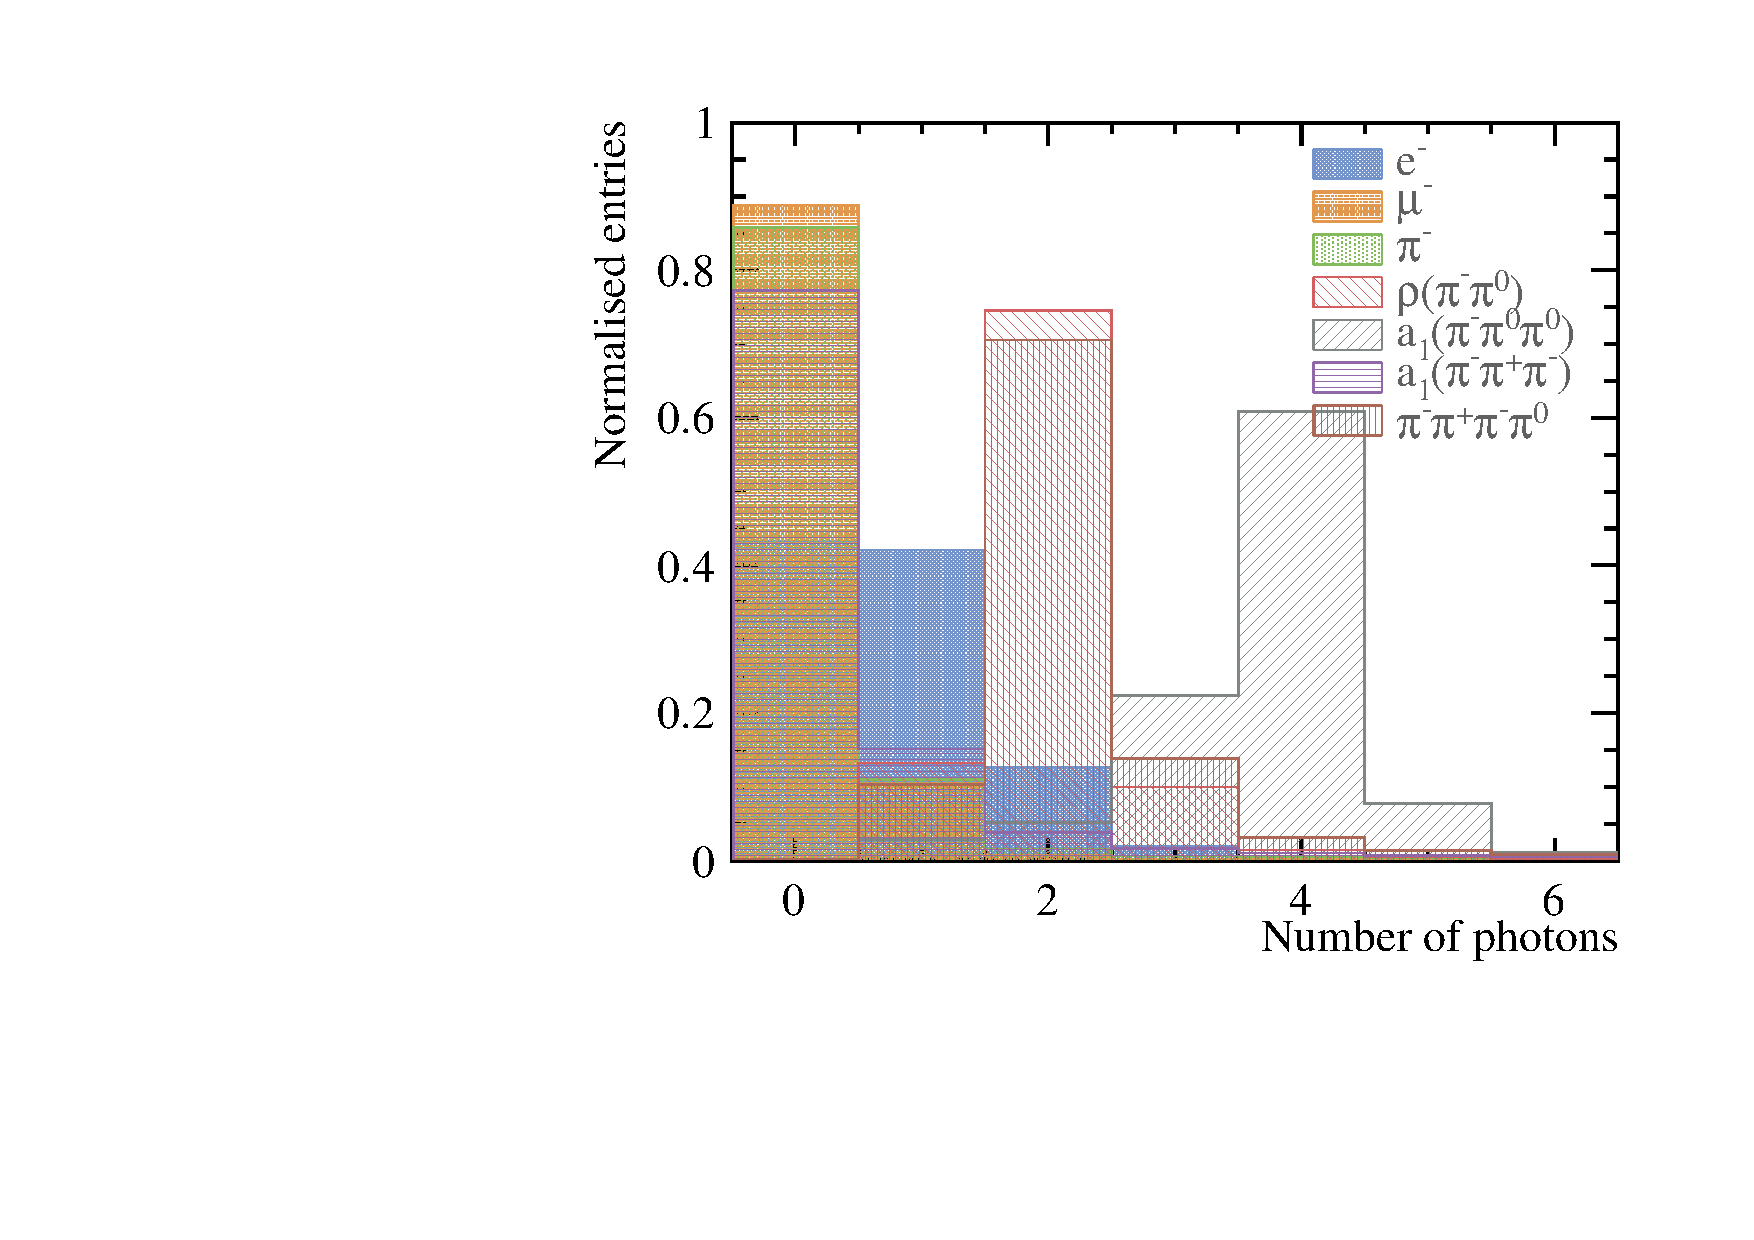
\includegraphics[width=.45\textwidth]{plots/var/nPhoton_100GeV_improved} 
\qquad
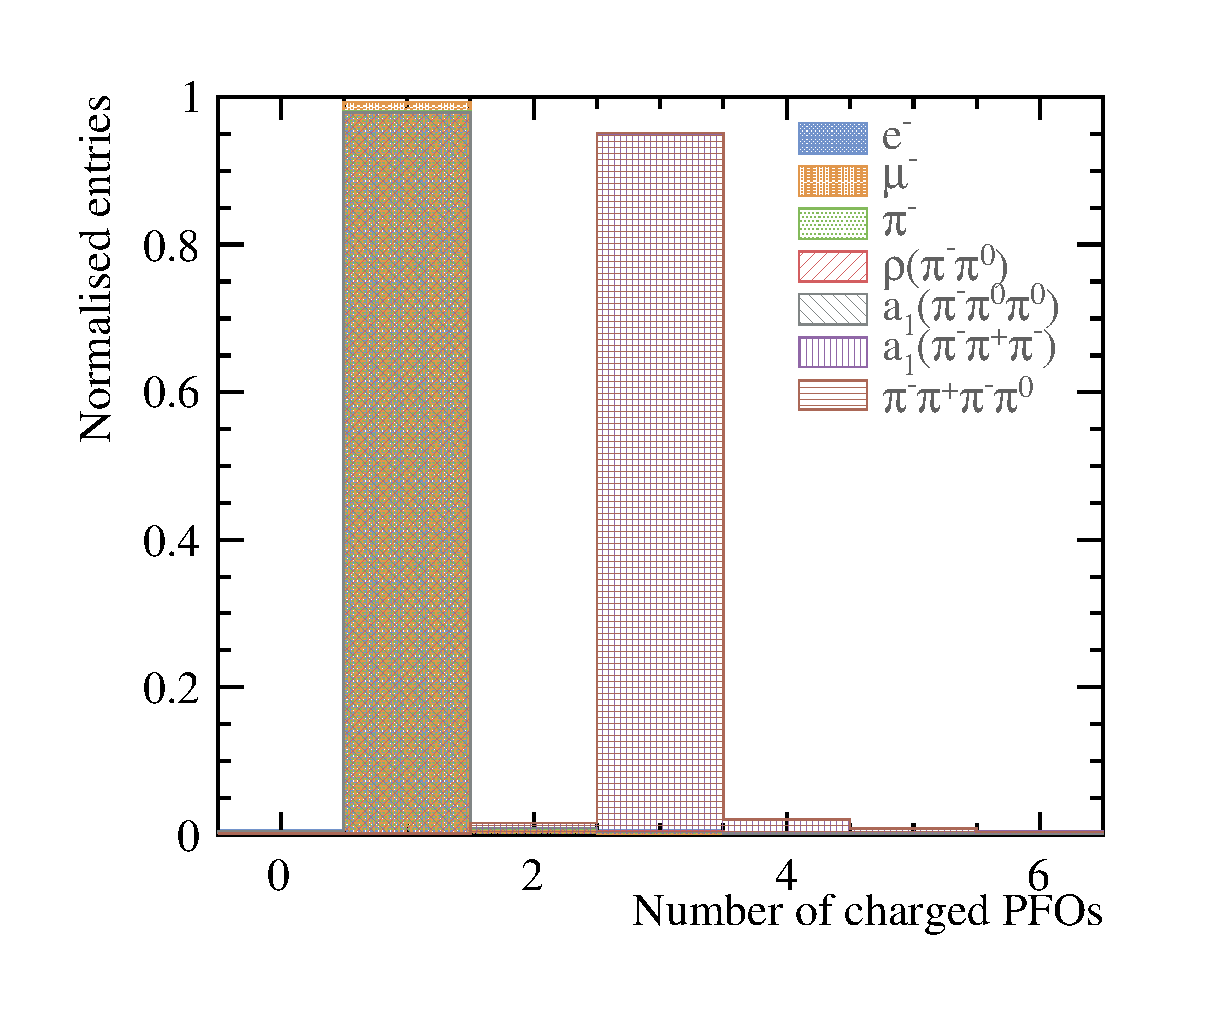
\includegraphics[width=.45\textwidth]{plots/var/nCharge_100GeV_improved} 
\qquad
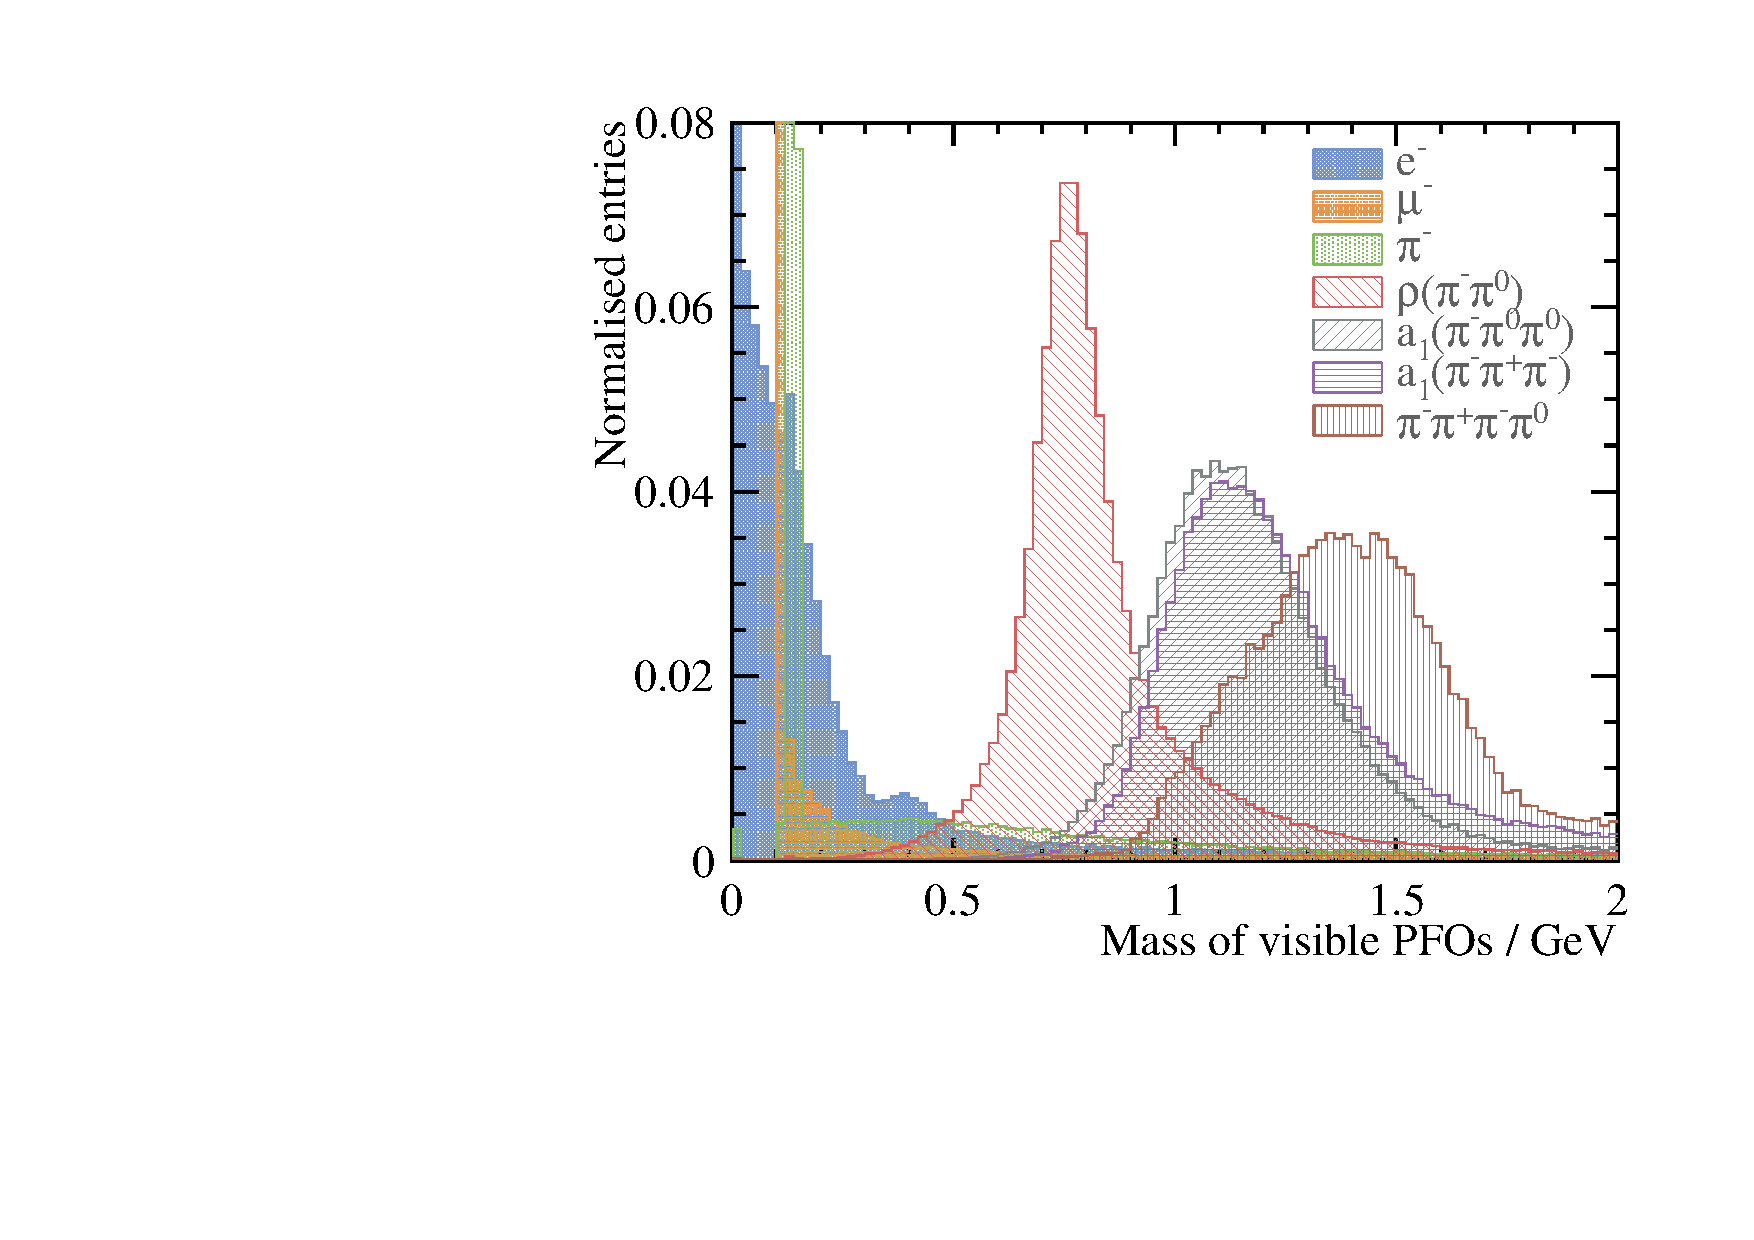
\includegraphics[width=.45\textwidth]{plots/var/mVis_100GeV_improved_zoom}
\qquad
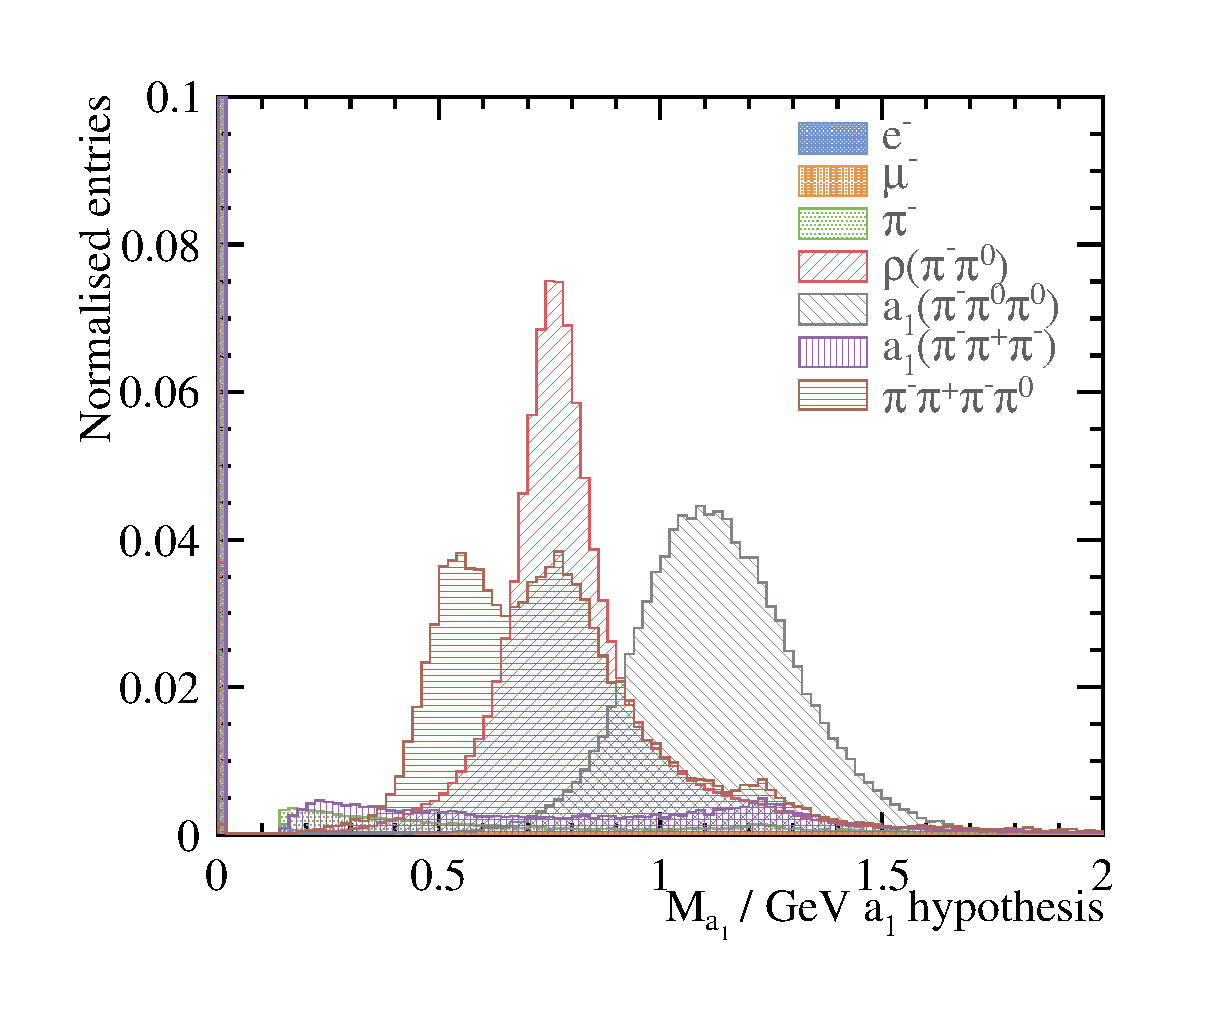
\includegraphics[width=.45\textwidth]{plots/var/mA1A1Fit_100GeV_improved_zoom}
\qquad

\caption{\label{fig:nPfos} 
The example normalised distribution for discriminative variables for seven final states, \decayElectron, \decayMuon, \decayPion, \decayRho, \decayAiPhoton, \decayAiPion and \decayThreePionPhoton, separated with truth information,  with \rootS = 100 \,GeV for nominal CLIC\_ILD detector model. The top left and top right, bottom left and bottom right plots are the normalised entries against the number of photons, number of charged PFOs, invariant mass of visible PFOs and the invariant mass of \decayAiPhotonShort for \decayAiPhotonShort hypothesis, respectively. There is a clear distinction between different final states in each plot.
}
\end{figure}


The first of variables separate final states into three broad categories: leptonic decays, one-prong with photons and three-prong with photons. The variables are the number of reconstructed PFOs of \PGmpm, \Pepm, \PGg, \PGppm and charged PFOs. As shown in figure~\ref{fig:nPfos}, there is a clear distinction between different final states. However, there is still  a lot of confusion between final states with multiple photons.

%From table~\ref{tab:decay_mode}, each final state has different number of \Pmupm, \Pepm, \Pphoton, \Ppipm and charged PFOs.
%If all PFOs were constructed perfectly, which is unrealistic, these varibles would be enough to separate different final states. %However the confusion between different final states could be minimised using other information.

The next set of varibles are designed to separate leptonic final states from the hadronic final states. Although leptonic final states have very different topologies to the hadronic state, i.e. \PGmpm deposits most energy in the muon chamber and some energy in the ECal and \Pepm deposited electromagnetic shower profile in the ECal, the difficulty is to correctly separate \Pepm from \PGppm, where \PGppm could start showering early in the ECal and be similar to a electromagnetic shower.

Varibles of interests are $\frac{\sum_{i}{E_{i,ECal}}}{\sum_{i}{E_{i,tot}}}$, $\frac{\sum_{c}{E_{c,ECal}}}{\sum_{c}{E_{c,tot}}}$, $\langle{E_{calo}}\rangle$, $\langle{d_{T}}\rangle$, $\langle{Layer_{L,start}}\rangle$, $\langle\Delta{Profile_{L}}\rangle$, $\frac{N_{MIP}}{N_{calo}}$,  $\langle{\frac{E_{c}}{P_{c}}}\rangle$ and  $\frac{E_{\Pmu}}{E_{\Ptau}}$, where $E_{ECal}$ is the energy deposited in the ECal,  $E_{tot}$ is the total energy deposited in the calorimeter, $i$ is summing over all PFOs, $c$ is summing over charged PFOs, $\langle{E_{calo}}\rangle$ is the the average energy of a calorimeter hit, $\langle{d_{T}}\rangle$ is the average transverse width of a cluster shower, $\langle{Layer_{L,start}}\rangle$ is the average longitudinal start layer of a cluster shower, $\langle\Delta{Profile_{L}}\rangle$ is the average discrepancy of a  cluster longitudinal shower profile to an electromagnetic shower profile, $\frac{N_{MIP}}{N_{calo}}$ is the fraction of calorimeter hits profiled as minimum ionising particles, $\langle{\frac{E_{c}}{P_{c}}}\rangle$ is the average ratio of the energy and the momentum of charged particles. $E_{\Pmu}$ is the energy of the reconstructed $\Pmupm$. 


 %$\frac{\sum_{c}{E_{c,ECal}}}{\sum_{c}{E_{c,tot}}}$ is above 0.95 and between 0.05 and 0.25 for \decayElectron and \decayMuon final states respectively and $\frac{N_{MIP}}{N_{calo}}$ is below 0.3 and above 0.8 for \decayElectron and \decayMuon final states respectively. Both are because \Pepm deposits most energy in the ECal and \PGmpm is minimally ionised in the ECal.  for  \Pepm because only \Pepm will deposit electromagnetic shower. $\langle{\frac{E_{c}}{P_{c}}}\rangle$ is mostly below 0.7 for \Pmupm final state because \Pmupm XX  $\langle\Delta{Profile_{L}}\rangle$ is below 0.05

 




For the hadronic decay final states, variables are $M_{PFOs}$, $M_{\Pphoton}$, $M_{\Ppipm}$, $M_{c}$, $M_{n}$, $\frac{E_{\Pphoton}}{E_{\Ptau}}$, $\frac{E_{\Ppipm}}{E_{\Ptau}}$ and $\frac{E_{c}}{E_{\Ptau}}$, where  $M_{PFOs}$, $M_{\Pphoton}$, $M_{\Ppipm}$, $M_{c}$, $M_{n}$ are the invariant masses of all PFOs, photons, charged pions, charged PFOs and neutral PFOs respectively, and $E_{\Pphoton}$, ${E_{\Ppipm}}$, ${E_{c}}$, $E_{\Ptau}$ are the energy of the $\Pphoton$, $\Ppipm$, charged particle and $\Ptau$ respectively. For final states with \PGr or \Pa resonance, the hypothesis tests are used. For example, for the \decayAiPhoton final state, the  $\chi_{\Pa}^{2}$ to minimise is,

\begin{equation}
\label{eq:a1}
\chi_{\Pa}^{2} = {\left(\frac{m_{\Pa,fit} -  m_{\Pa}}{\sigma_{\Pa}}\right)}^{2} + {\left(\frac{{m_{\PGpz,fit}} -  m_{\PGpz}}{\sigma_{\PGpz}}\right)}^{2} + {\left(\frac{{m_{\PGpz^*,fit}} -  m_{\PGpz}}{\sigma_{\PGpz}}\right)}^{2}  \,,
\end{equation}

where $m_{\PGpz,fit}$ and $m_{\PGpz^*,fit}$  are the invariant masses of all possible two photons combinations, $\sigma_{\Pa}$ and $\sigma_{\PGpz}$ are the half width of the invariant mass distribution of reconstructed \Pa and \PGpz using the truth information, and $m_{\Pa}$ and $m_{\PGp}$ are the masses of \Pa and \PGpz, taken from \cite{Agashe:2014kda}. If there are two or three photons, the $\chi_{\Pa}^{2}$ expression will be reduced and not including $m_{\PGpz^*,fit}$ term. If there are fewer than two photons, the $\chi_{\Pa}^{2}$ expression would only contain $m_{\Pa,fit}$ term.


For the \decayRho final state, a similar $\chi_{\PGr}^{2}$ test for \PGr hypothesis is used to extract $m_{\PGr,fit}$ and $m_{\PGpz,fit}$ variables. $\chi_{\PGr}^{2}$ is similar to $\chi_{\Pa}^{2}$ with \PGr replacing \Pa and only one $m_{\PGpz,fit}$ term.


Figure~\ref{fig:nPfos} shows the $m_{\Pa,fit}$ where \decayRho, \decayAiPhoton  and \decayThreePionPhoton final states contribute to the \Pa resonance, although only \decayAiPhoton final has a real \Pa resonance. This is due to the structure of the  $\chi_{\Pa}^{2}$ minimisation function allowing final states with more than two photons and one \PGppm to contribute.





%, listed in Table XX. Note that XX variables were specialised in separating a electron from a pion. XX variables were made to test the hypothesis of XX particles. The rho hypothesis is to find the best rho decay candidates by minimising chi squared according to $aa$, where X is all possible charge pions, Y is all possible 2 photons. The formula will reduce accordingly if there is 1 photon. Similarly, the a1 decaying to 1 pion 4 photon hypothesis is done in a same fashion with Chi squared function XX, , where X is all possible charge pions, Y is all possible 2 photons. The formula will reduce accordingly if there are 2 or 3 photons.

Energy of the \PGt is assume to be the same as the energy of \Pepm beam, which is half of the \rootS energy. Recoil momenta were calculated assuming the \Pem\Pep collision happened at the centre of mass energy. Both assumptions are largely valid when there is no ISR contribution. %The variables of energy ratios instead of the raw energies were calculated to make the MVA process more generic across different c.o.m. energies.

For the multivariate analysis, the multiclass class of the TMVA package \cite{Therhaag:2009dp} was used to train the seven final states simultaneously. The multiclass class is an extension of the standard signal-background classifier. For each final state, the multiclass classifier will train the final state as the signal against all other final states as the background. This process is repeated for each final state. The classifier output for a single event is a normalised number for each final state, where the sum is one. The number of a final state of a event can be used as the probability. The event is classified into a particular final state if the final state has the highest classifier output number. The advantage of using the multiclass is that the correction between different final states are accounted for and the classifier output are correctly adjusted for multiple final states, hence one event can only be classified into one final state.

Half of the randomly selected samples were used in the training process and the other half were used for testing. 

The TMVA multiclass classifier used is boosted decision tree with gradient boosting (BDTG), as it was found to give for the best performance. The MVA classifier is trained and optimised to give the best overall separation across all final states.

\section{Results and discussion}

\begin{table}[htbp]
\centering
\caption{\label{tab:sel_example} The probability of reconstruction of true decay modes in columns in percent, with \rootS = 100 \,GeV for nominal CLIC\_ILD detector model. Bold numbers show the correctly reconstructed terms. Numbers less than 0.25\% are not shown. Statistical uncertainties are less than 0.25\%. Final states include \PGnGt, which is not shown.}
\smallskip
\small
\begin{tabular}{| l | r | r | r | r | r | r | r |}
\hline
  \textbf{Reco $\downarrow$ True $\to$}  & \textbf{\decayElectronShort} & \textbf{\decayMuonShort} &\textbf{\decayPionShort} & \textbf{\decayRhoShort} &\textbf{\decayAiPhotonShort} &\textbf{\decayAiPionShort} &\textbf{\decayThreePionPhotonShort} \\
\hline

\textbf{\decayElectronShort}&\boldmath{99.8}&-&0.9&1.1&0.8&-&-\\
\textbf{\decayMuonShort}&-&\boldmath{99.5}&0.5&-&-&-&-\\
\textbf{\decayPionShort}&-&0.3&\boldmath{93.2}&0.9&-&0.4&-\\
\textbf{\decayRhoShort}&-&-&4.1&\boldmath{93.0}&10.5&0.6&2.8\\
\textbf{\decayAiPhotonShort}&-&-&-&4.3&88.2&-&1.0\\
\textbf{\decayAiPionShort}&-&-&1.0&0.3&-&\boldmath{96.6}&6.9\\
\textbf{\decayThreePionPhotonShort}&-&-&-&0.4&0.4&2.4&\boldmath{89.3}\\

\hline
\end{tabular}
\end{table}

The reconstruction efficiencies for the seven final state of the tau decaying with c.o.m. energy of 100 \,GeV for the nominal CLIC\_ILD detector are shown in the table~\ref{tab:sel_example}.

The study was repeated with  \rootS = 100, 200, 500, 1000 GeV. The ECal square cell sizes were also varied at 3, 5, 7, 10, 15 and 20\,mm, whilst keeping the the total ECal size the same. The results table were are in the appendix X. 

\begin{figure}[htbp]
\centering % \begin{center}/\end{center} takes some additional vertical space
%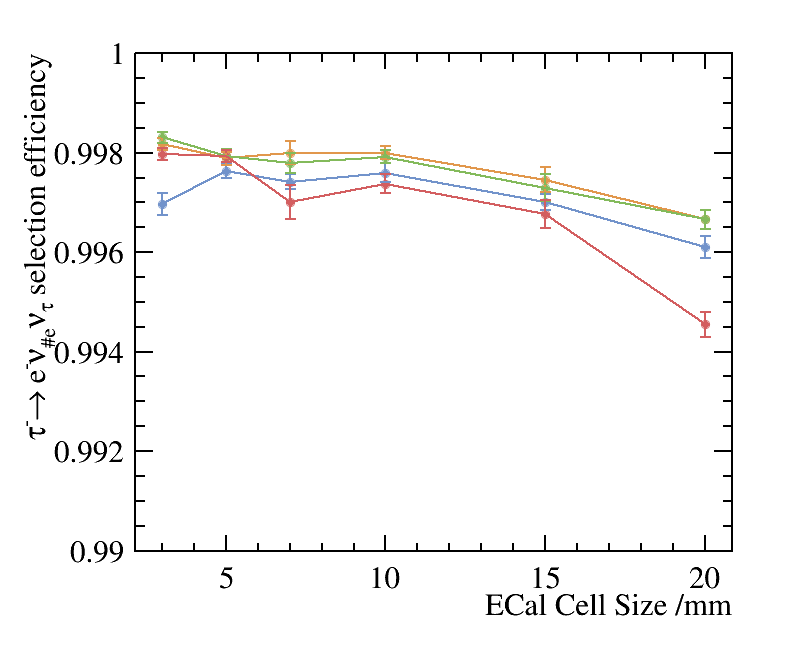
\includegraphics[width=.45\textwidth]{plots/decayMode0} 
%\qquad
%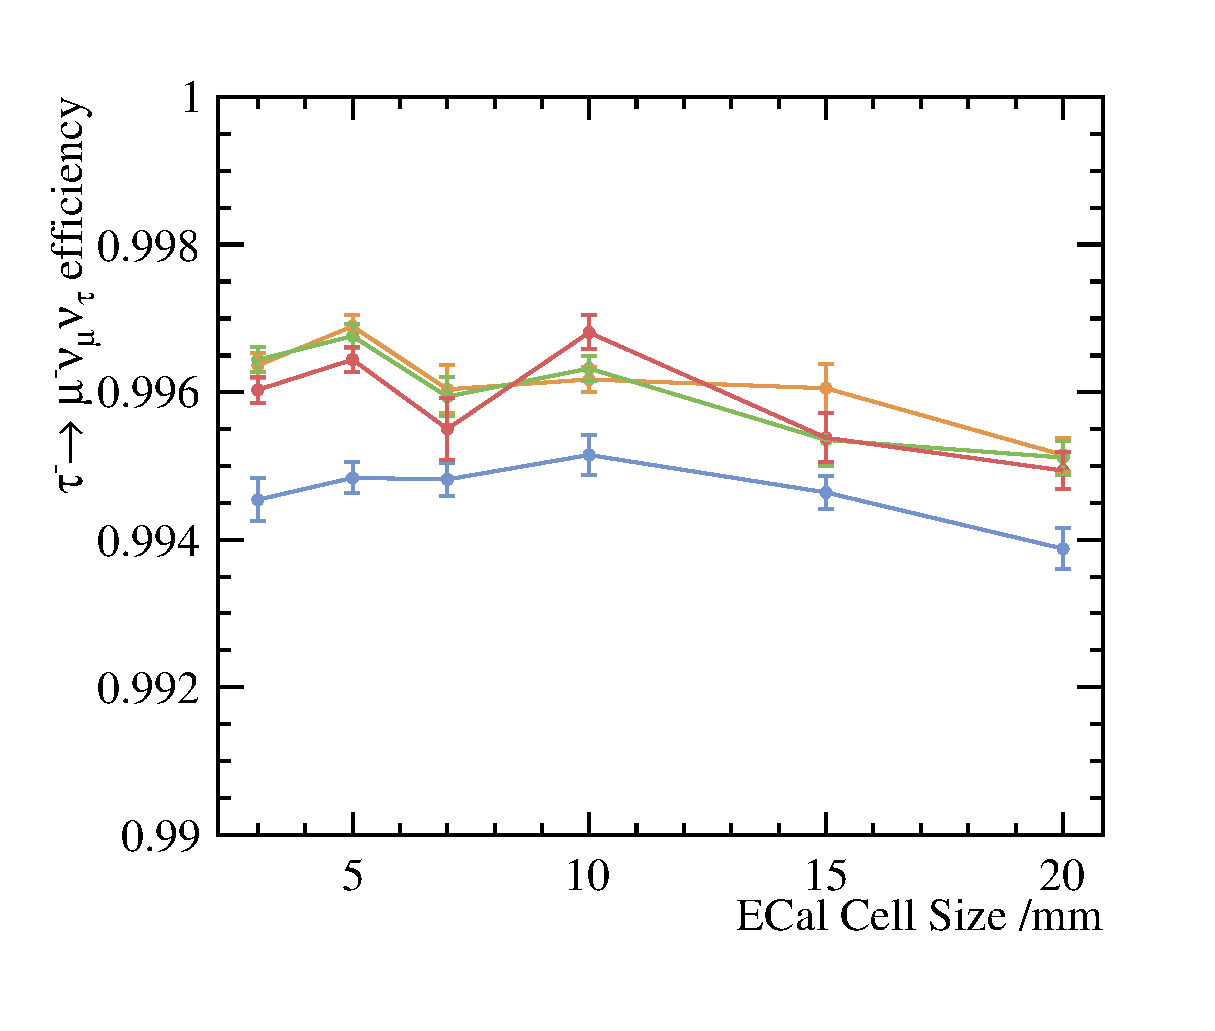
\includegraphics[width=.45\textwidth]{plots/decayMode1} 
%\qquad
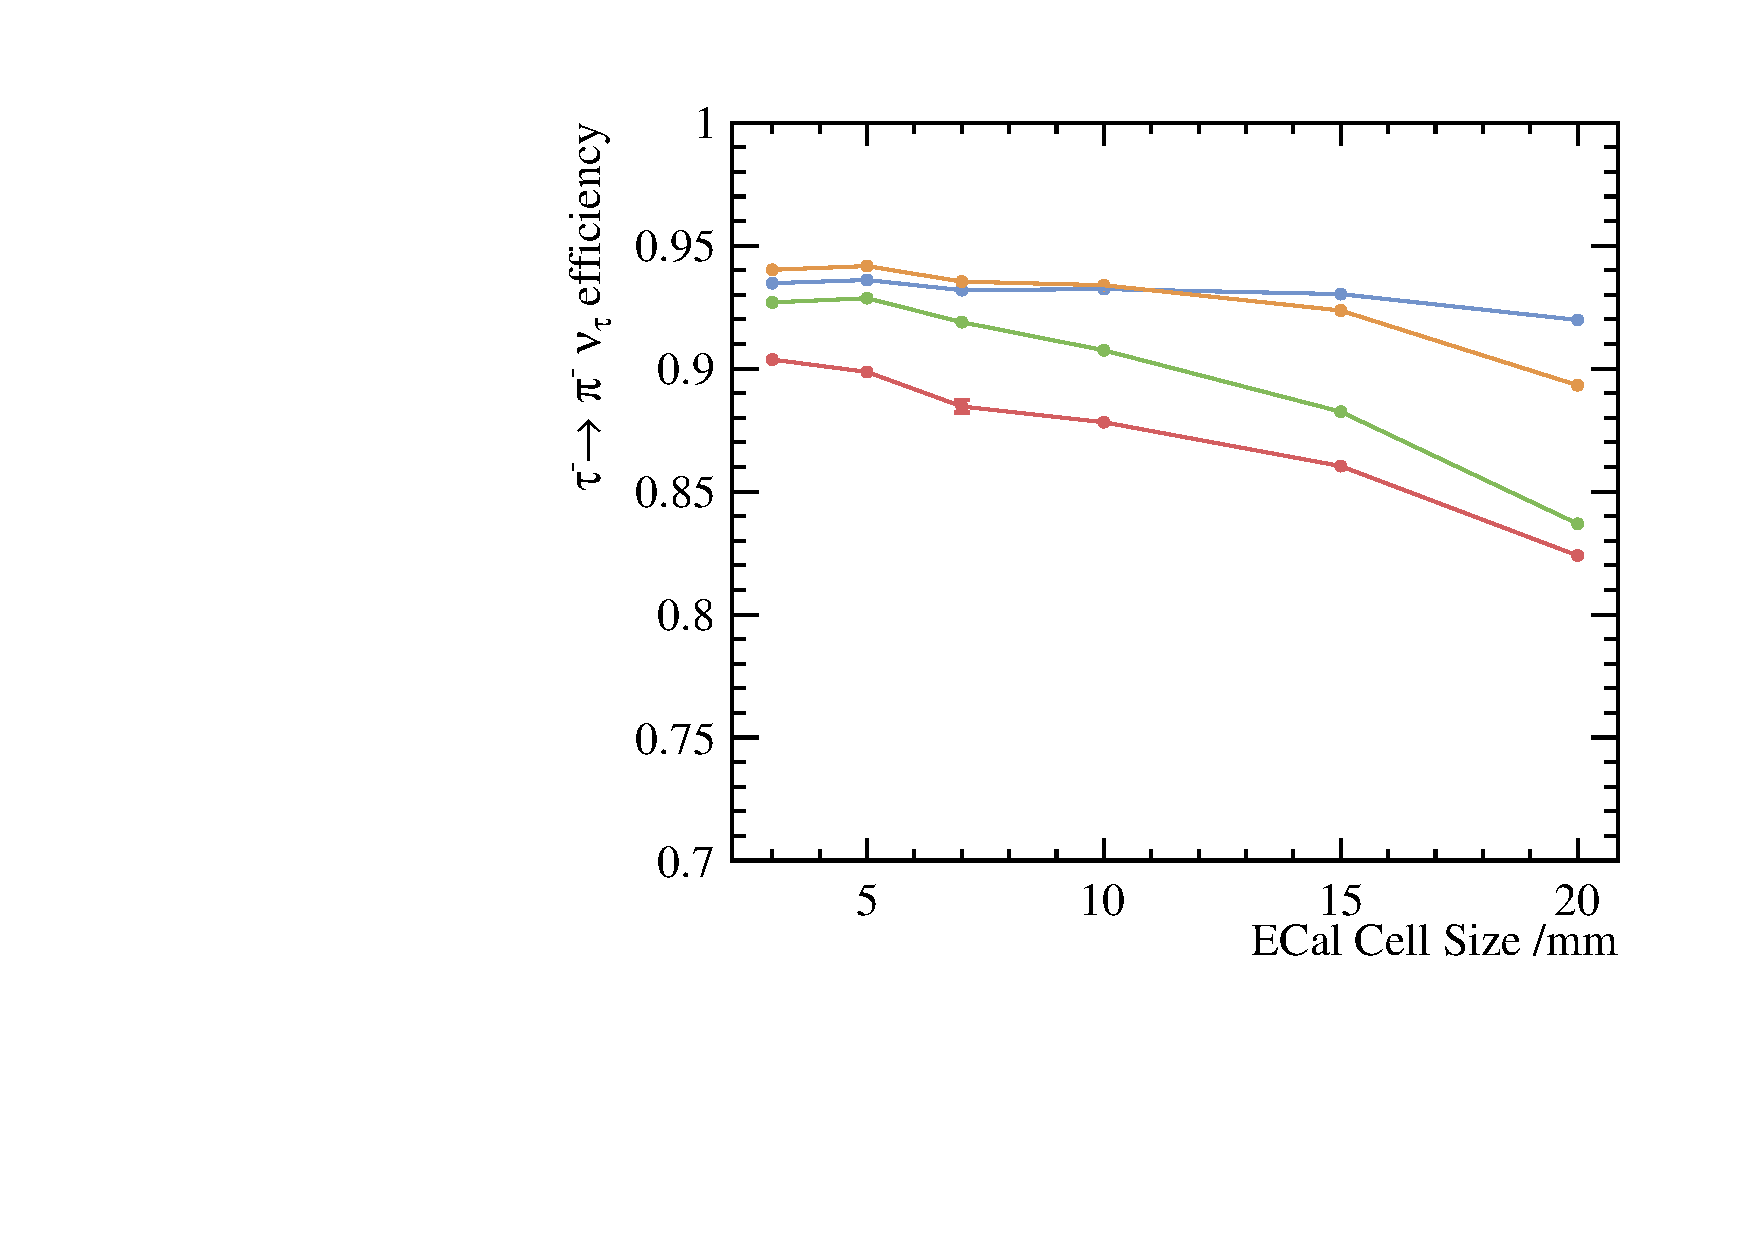
\includegraphics[width=.45\textwidth]{plots/decayMode2}
\qquad
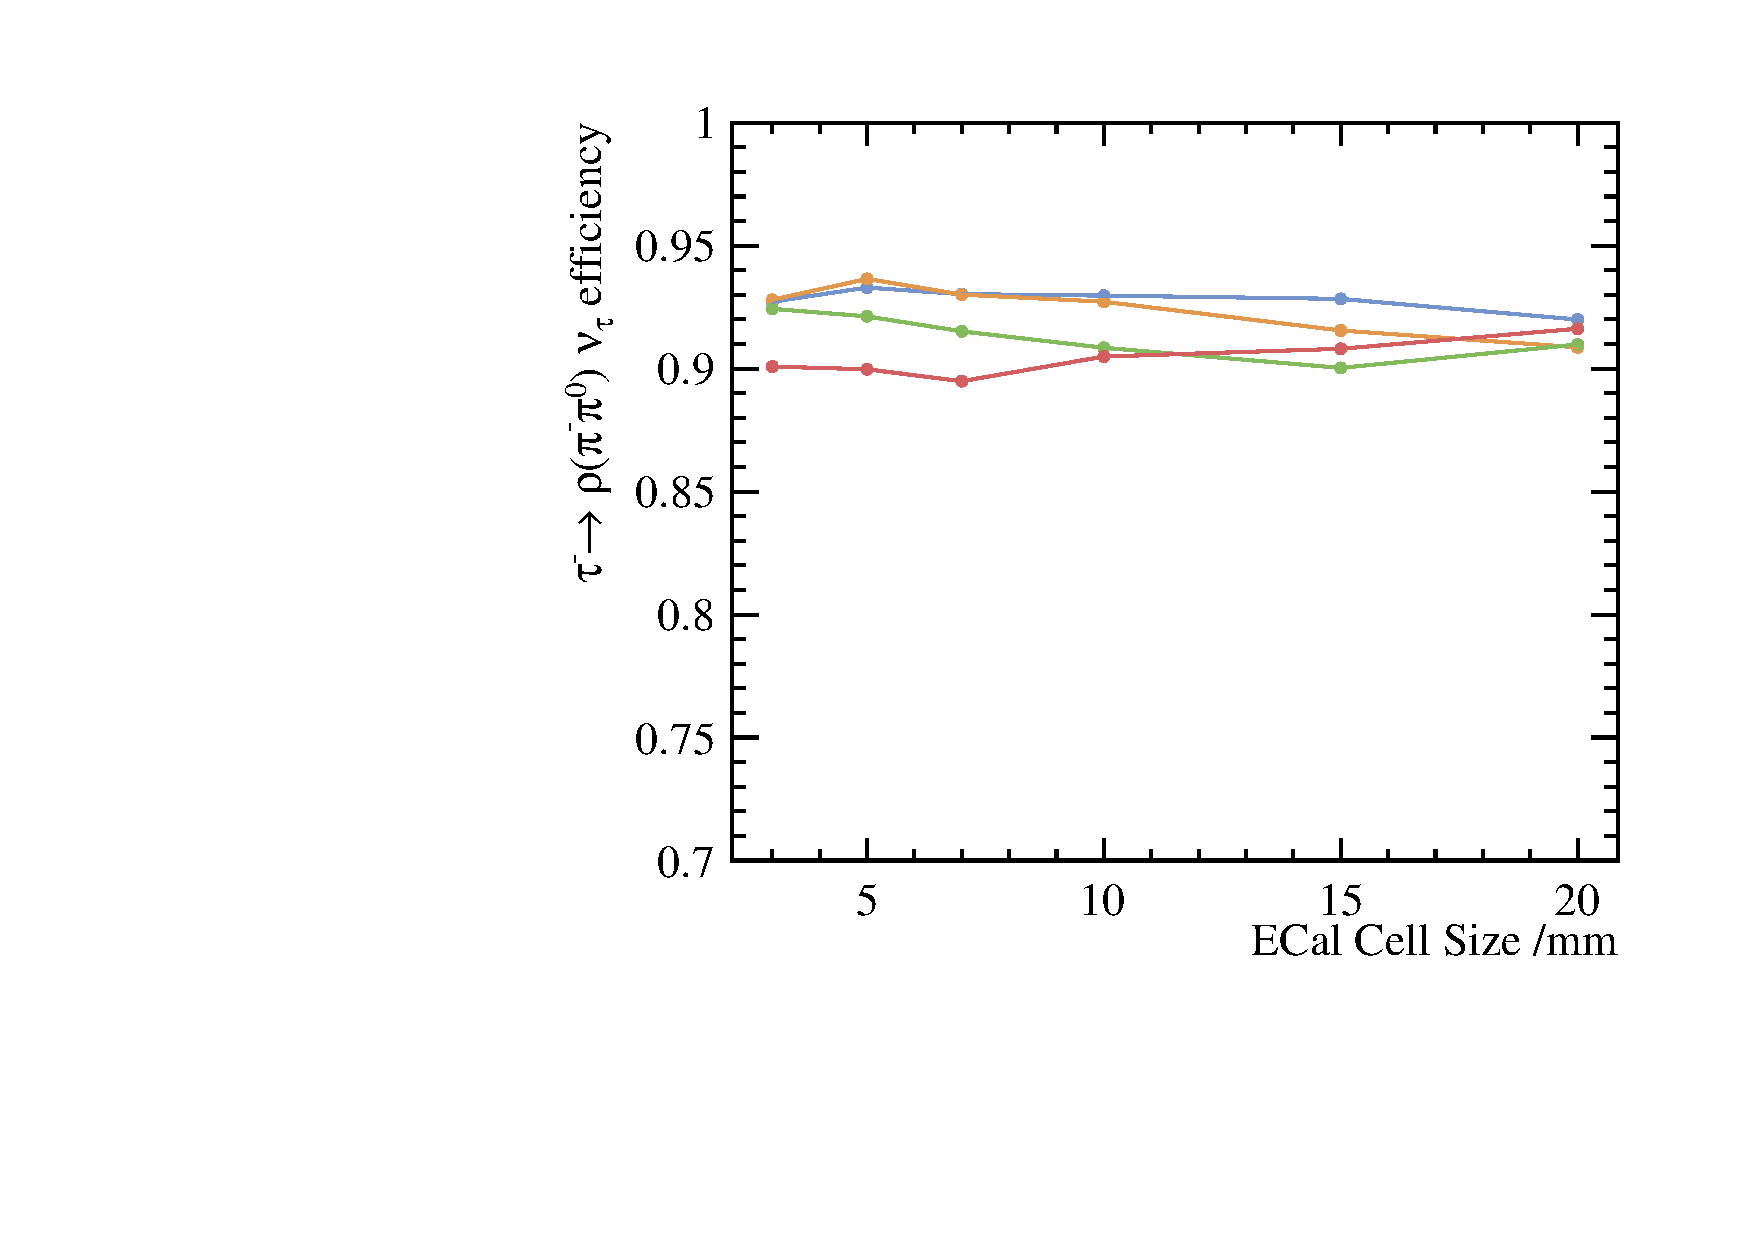
\includegraphics[width=.45\textwidth]{plots/decayMode3} 
\qquad
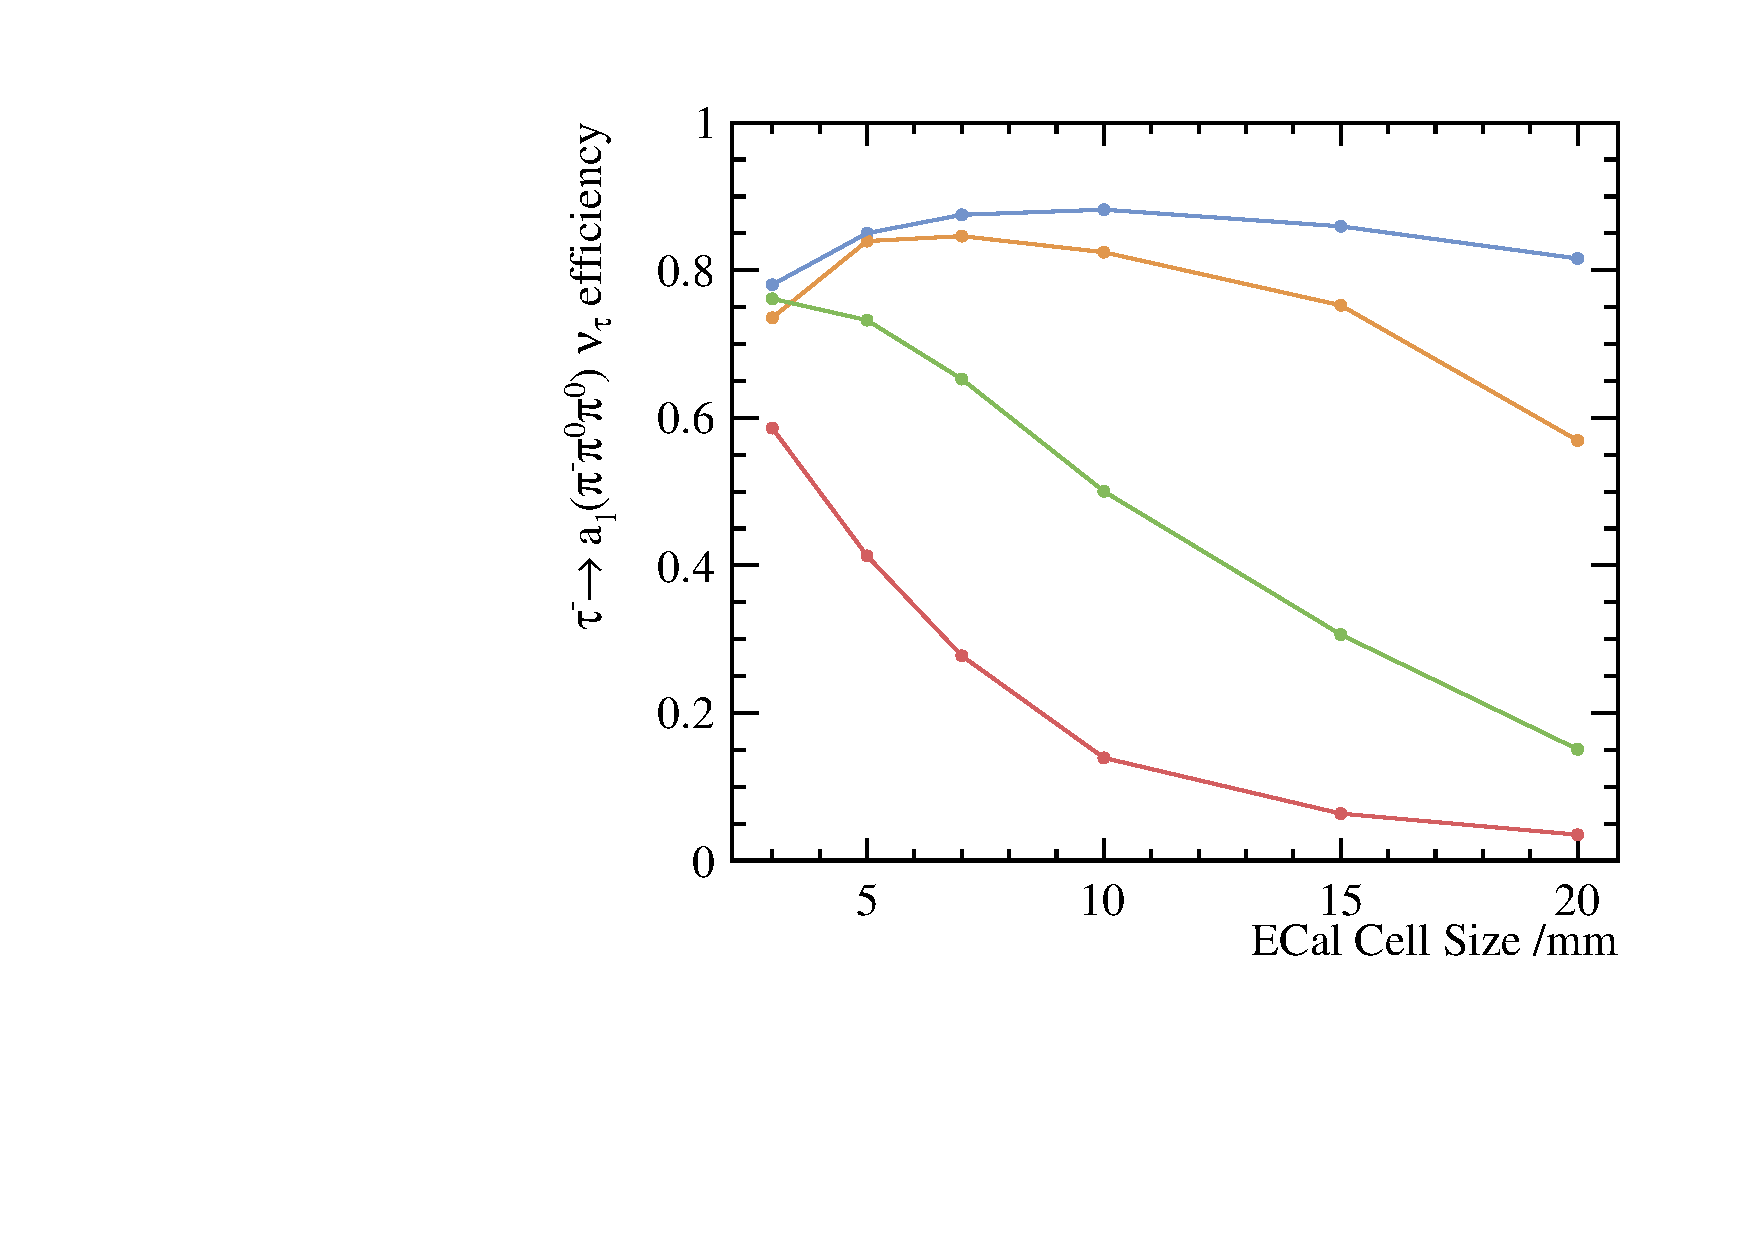
\includegraphics[width=.45\textwidth]{plots/decayMode4} 
\qquad
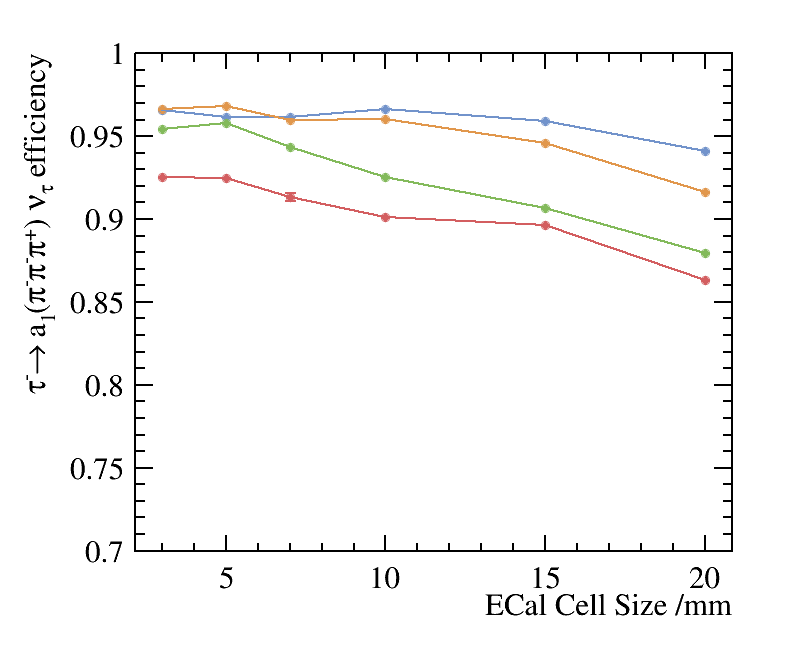
\includegraphics[width=.45\textwidth]{plots/decayMode5}
\qquad
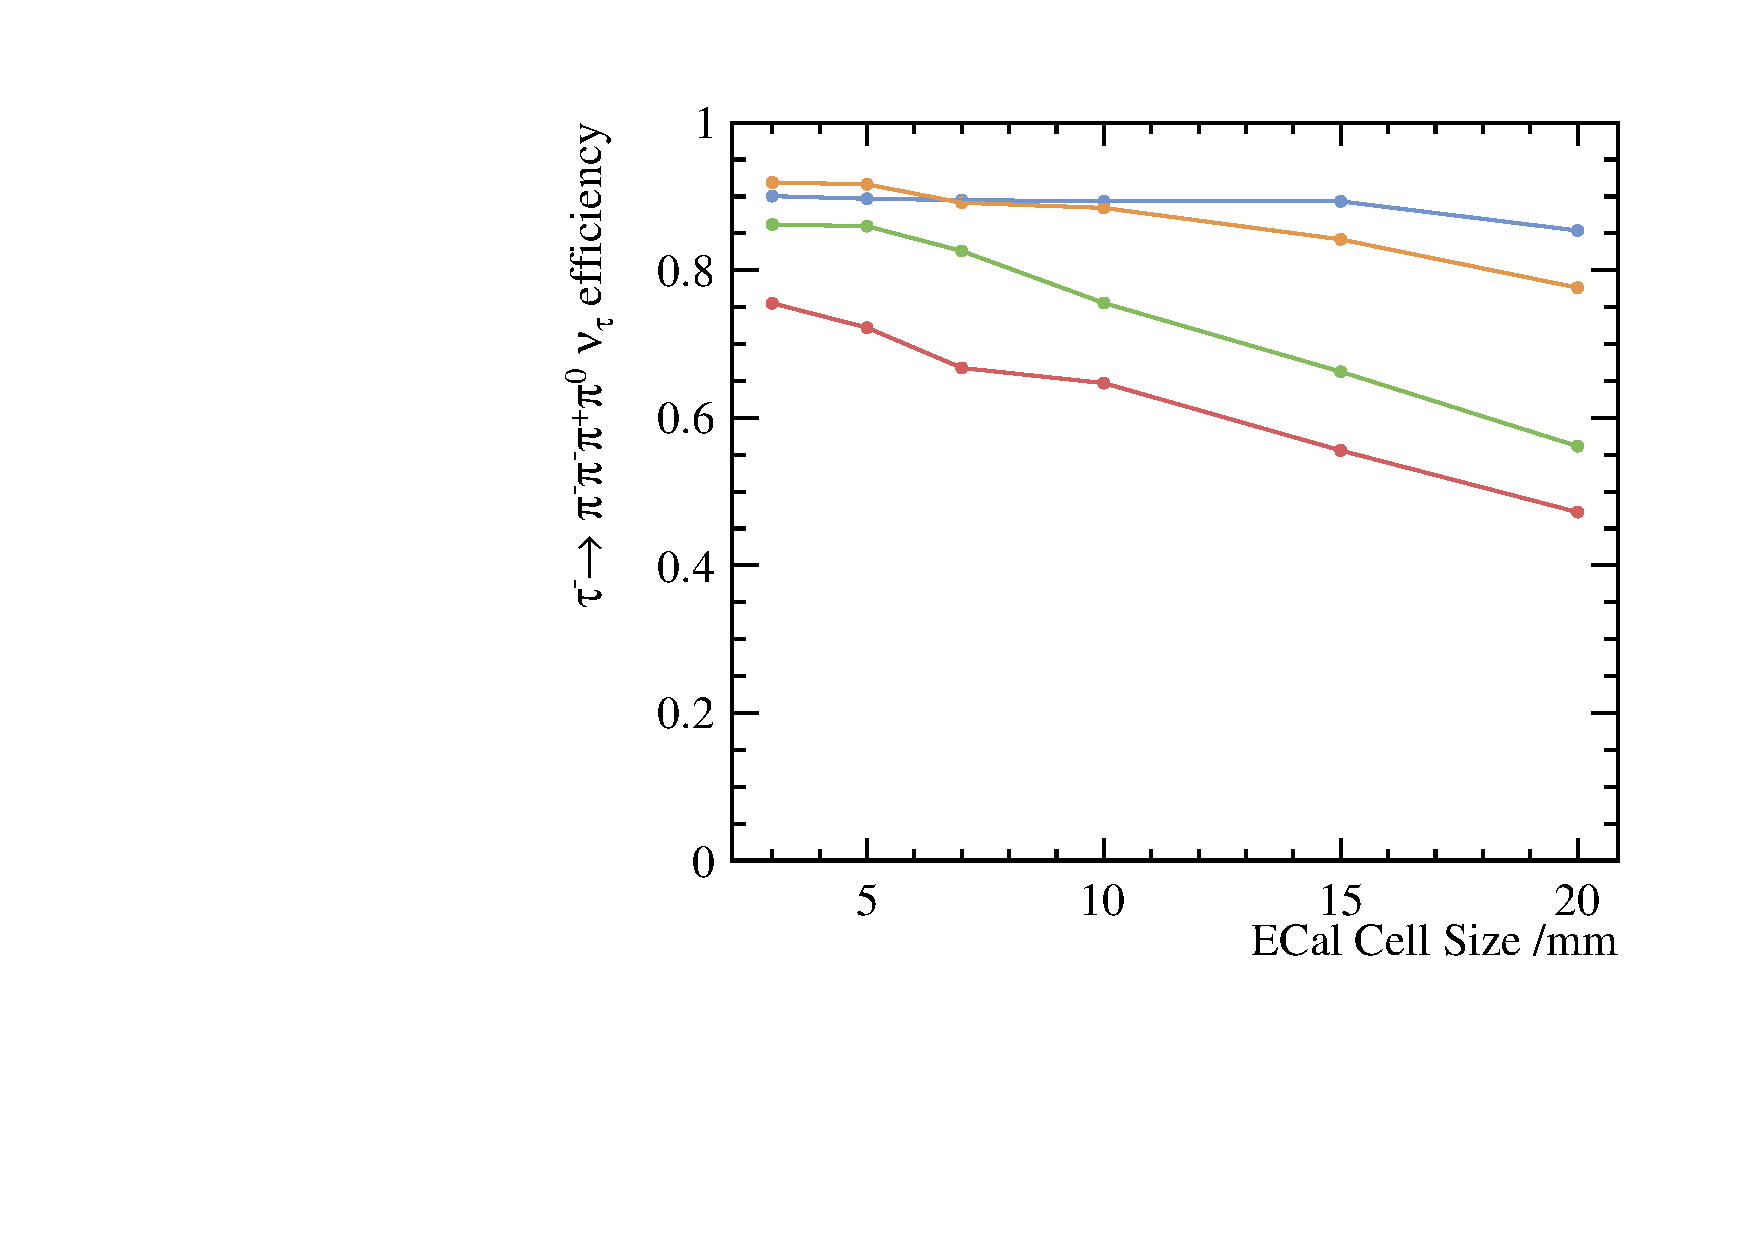
\includegraphics[width=.45\textwidth]{plots/decayMode6}
\qquad
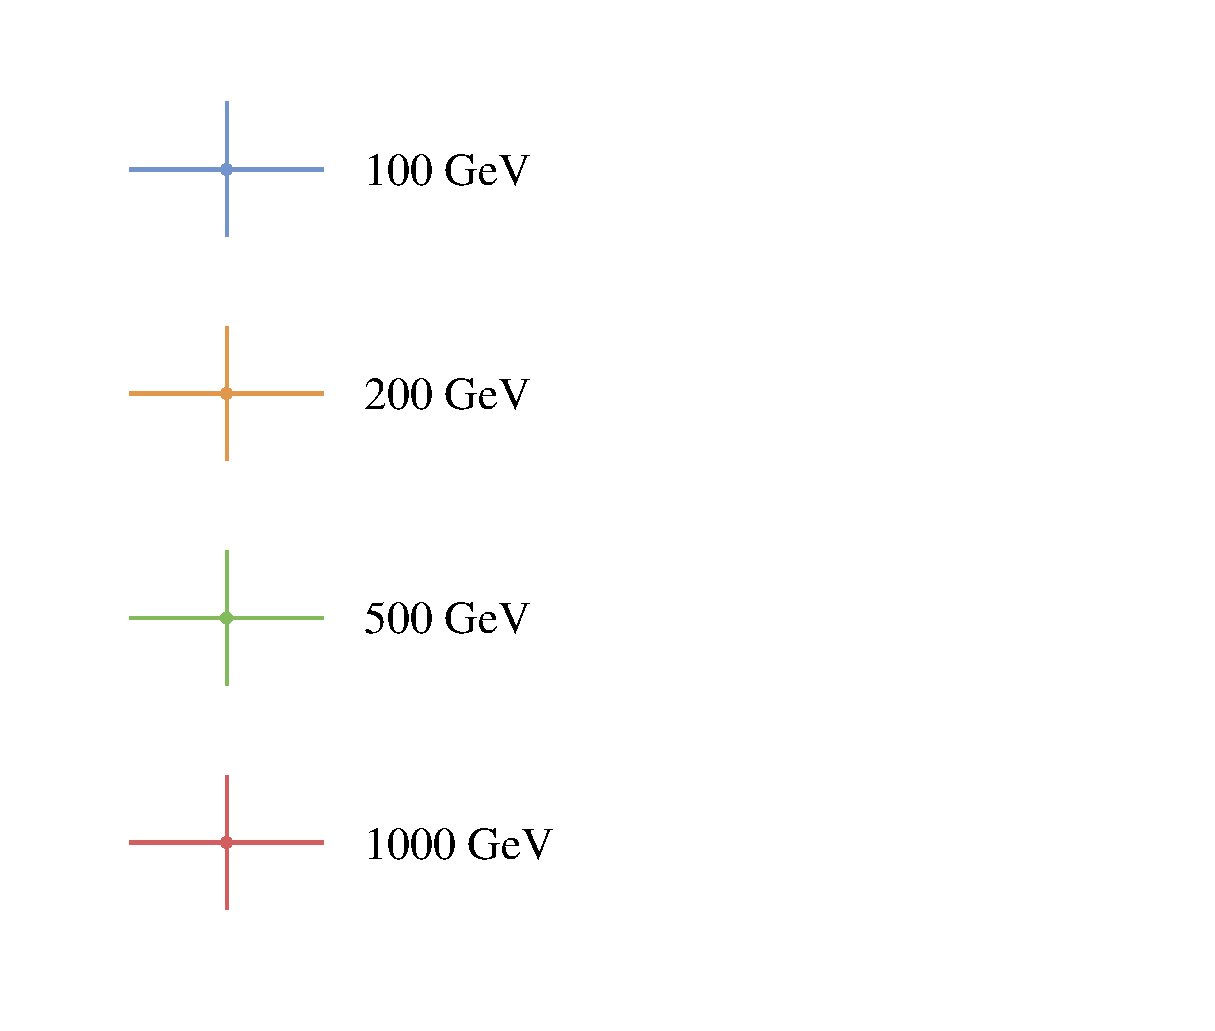
\includegraphics[width=.45\textwidth]{plots/legend}
%\qquad
%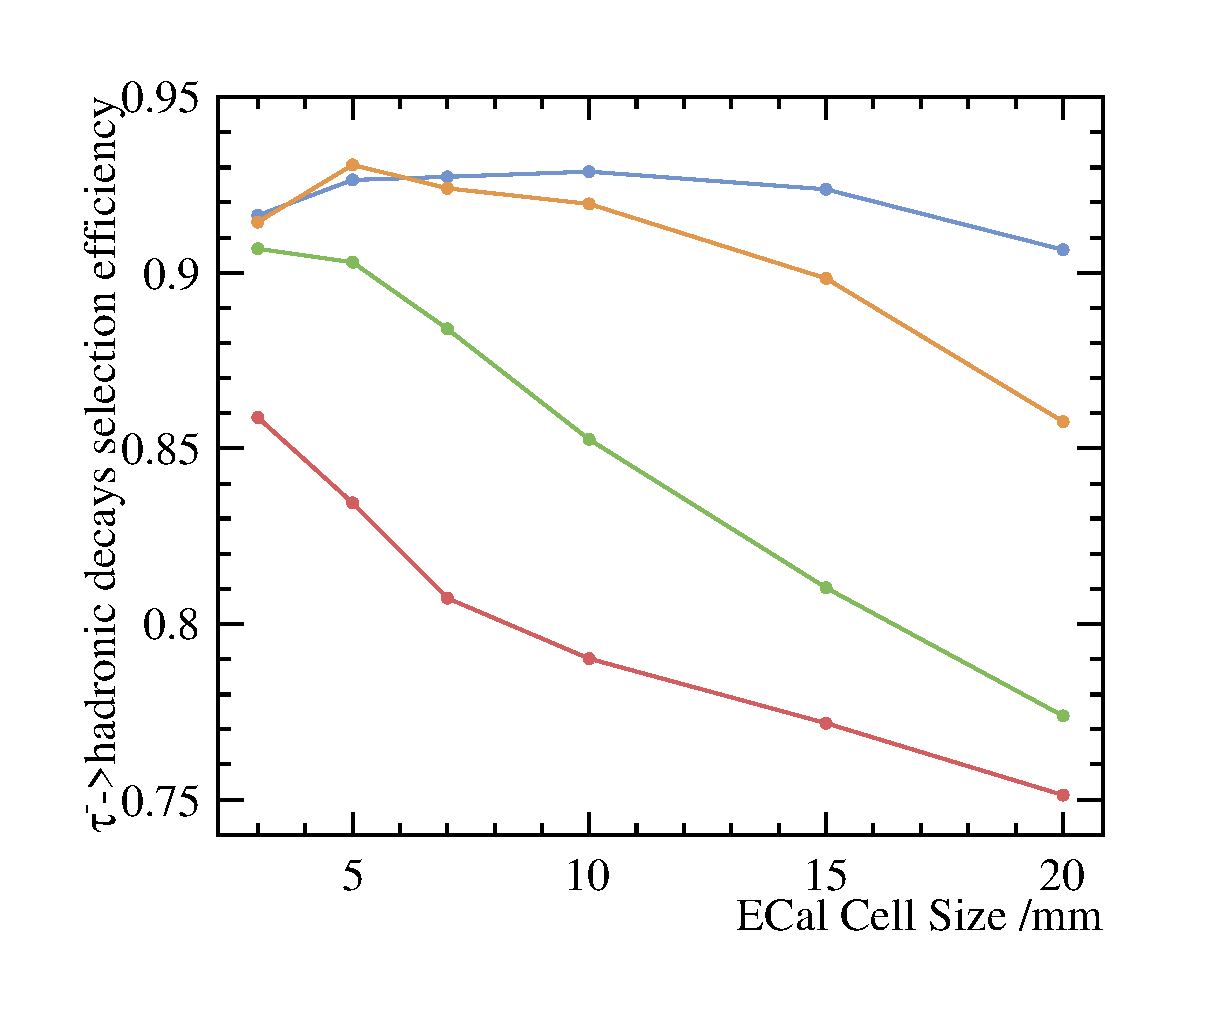
\includegraphics[width=.4\textwidth]{plots/hadEff}
% "\includegraphics" from the "graphicx" permits to crop (trim+clip)
% and rotate (angle) and image (and much more)
\caption{\label{fig:pion_efficiency} The selection efficiencies for various final states against the ECal cell size for different c.o.m. energies with the nominal CLIC\_ILD detector model are shown. The top left, top right, middle left, middle right and bottom left plots are for the \decayPion, \decayRho,  \decayAiPhoton, \decayAiPion  and \decayThreePionPhoton  final states respectively. From the top to the bottom, blue, orange, green and red lines are representing the \rootS = 100, 200, 500 and 1000\,GeV respectively. Note that the y axis are not the same for displaying purpose.}
\end{figure}

To compare the impact of the ECAL cell sizes and the \rootS energies on the separation of tau final states, the selection efficiencies were plotted in the figure~\ref{fig:pion_efficiency}. The leptonic decay selection efficiencies are not shown as they are similar across different ECal cell sizes. This is because the \Pepm and \PGmpm identifications mostly rely on the tracking system, which was not varied in this study. The energy deposited in the calorimeter are used for the association to the tracks but it has a small impact on the lepton identification. 

Overall, the hadronic decay selection efficiency decreases as the \rootS energy increases. This is due to the fact that when {\PGt}s are boosted at higher \rootS energies, the separation between decay products is smaller. Hence it is more difficult to reconstruct multi-photon final states correctly.

As the ECal cell sizes increase, the reconstruction efficiencies generally decrease. Larger cell sizes have lower spatial resolutions, making the separating of nearby photons more difficult.

For the \decayAiPhoton final state, the selection efficiency for 500\,GeV rises from ECal cell sizes 15\,mm to 20\,mm and the one for 1000\,GeV rises from 7\,, to 20\,mm actually goes up as cell size increases. This is because when the algorithm can not reconstruct four photons in the \decayAiPhoton final state, and the event topology would be very similar to the \decayRho final states. 

For the \rootS = 100 and 200\,GeV, the selection efficiency of the 5\,mm ECal cell size is better than that of the 3\,mm. One possible explanation is that the  and the PandoraPFA have been optimised for the nominal ILD detector with the 5\,mm ECal cell size, which shares the same ECal structure with the nominal CLIC\_ILD detector.

\begin{figure}[htbp]
\centering % \begin{center}/\end{center} takes some additional vertical space
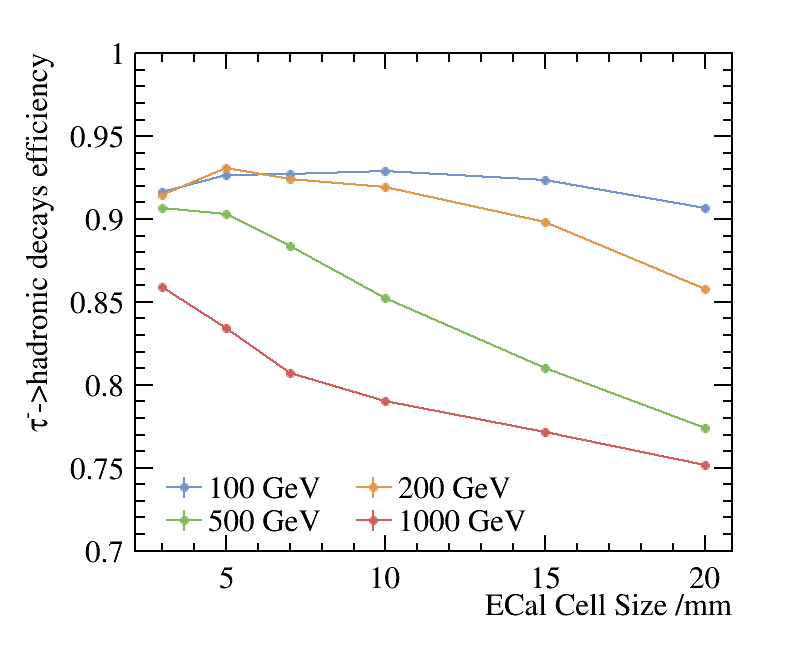
\includegraphics[width=.45\textwidth]{plots/hadronicEff}
% "\includegraphics" from the "graphicx" permits to crop (trim+clip)
% and rotate (angle) and image (and much more)
\caption{\label{fig:hadronic_efficiency} The \PGt hadronic decay selection efficiency against the ECal cell size for different \rootS energies with the nominal CLIC\_ILD detector model are shown. The blue, orange, green and red lines are representing the \rootS = 100, 200, 500 and 1000\,GeV respectively.}
\end{figure}

In order to compare the overall separation power of all the final states across c.o.m. energy and the ECal cell sizes, we constructed a single parameter function, the  \PGt hadronic decay final state efficiency function, 
\begin{equation}
\label{eq:had}
\varepsilon_{had} = \frac{\left(\Sigma_{i} {Br}_{i}\varepsilon_{i}\right)}{\Sigma_{i} {Br}_{i}}  \,,
\end{equation}
where $Br_{i}$ is the branching fraction of a hadronic final state after the generator level cut, $\varepsilon_{i}$ is the selection efficiency of the final state and the $i$ is summing over five hadronic decay final state of \PGt. Leptonic decays, \decayElectron and \decayMuon, were not included as the variation of the leptonic decay selection efficiency is small.

In the figure~\ref{fig:hadronic_efficiency}, \PGt hadronic decay final state efficiency, $\varepsilon_{had}$, against the ECal cell size with different \rootS is shown. $\varepsilon_{had}$ decreases when cell sizes increases and when \rootS increases.  Again, $\varepsilon_{had}$ of the 5\,mm ECal cell size is better than that of the 3\,mm for 100 and 200\,GeV lines possibly due the optimisation of the software fro the nominal ILD 5\,mm cell size.

The $\varepsilon_{had}$ is above 90\% for the ECal cell size from 3 to 20\,mm for the \rootS = 100\,GeV. For \rootS = 200\,GeV, the $\varepsilon_{had}$ decreases from over 90\% to 86\% for the ECal cell size from 3 to 20\,mm. The degradation of the $\varepsilon_{had}$ is significant for the 500 and 1000\,GeV lines, where the $\varepsilon_{had}$ drops from over 90\% to 77\%  and from 86\% to 75\% respectively. 

For low \rootS, namely 100 and 200\,GeV, up to 15\,mm cell sizes of ECal will give a good performance for \PGt hadronic decay modes separation, and the $\varepsilon_{had}$ is above 90\%. For the high c\rootS, namely 500 and 1000\,GeV, it is preferential to have a small ECal cell size for \PGt hadronic decay modes separation. There is about 15\% degradation of $\varepsilon_{had}$ for ECal cell size from 3 to 20\,mm.

%The degradation of $\varepsilon_{hadronic}$ is more significant for higher c.o.m. energy.

The paper illustrated the usage of reconstruction of the tau decay modes as a benchmark for the detector optimisation. 

%The high probability of correctly identifying the decay modes also showed the potential to measure the spin of the {\Ptau} with the CLIC machine.


%We discourage the use of inline figures (wrapfigure), as they may be
%difficult to position if the page layout changes.

%We suggest not to abbreviate: ``section'', ``appendix'', ``figure''
%and ``table'', but ``eq.'' and ``ref.'' are welcome. Also, please do
%not use \texttt{\textbackslash emph} or \texttt{\textbackslash it} for
%latin abbreviaitons: i.e., et al., e.g., vs., etc.



%\section{Sections}
%\subsection{And subsequent}
%\subsubsection{Sub-sections}
%\paragraph{Up to paragraphs.} We find that having more levels usually
%reduces the clarity of the article. Also, we strongly discourage the
%use of non-numbered sections (e.g.~\texttt{\textbackslash
%  subsubsection*}).  Please also see the use of
%``\texttt{\textbackslash texorpdfstring\{\}\{\}}'' to avoid warnings
%from the hyperref package when you have math in the section titles



%\appendix
%\section{Some title}
%Please always give a title also for appendices.


\acknowledgments

The authors would like to thank P. G. Roloff for helping to generate the simulated samples. 

%\paragraph{Note added.} This is also a good position for notes added
%after the paper has been written.





% We suggest to always provide author, title and journal data:
% in short all the informations that clearly identify a document.

\bibliographystyle{h-physrev3}
\bibliography{bib}

%\begin{thebibliography}{99}

%\bibitem{a}
%Author, \emph{Title}, \emph{J. Abbrev.} {\bf vol} (year) pg.

%\bibitem{b}
%Author, \emph{Title},
%arxiv:1234.5678.

%\bibitem{c}
%Author, \emph{Title},
%Publisher (year).


% Please avoid comments such as "For a review'', "For some examples",
% "and references therein" or move them in the text. In general,
% please leave only references in the bibliography and move all
% accessory text in footnotes.

% Also, please have only one work for each \bibitem.


%\end{thebibliography}
\end{document}
